%%%%%%%%%%%%%%%%%%%%%%%%%%%%%%%%%%%%%%%%%
% Thin Sectioned Essay
% LaTeX Template
% Version 1.0 (3/8/13)
%
% This template has been downloaded from:
% http://www.LaTeXTemplates.com
%
% Original Author:
% Nicolas Diaz (nsdiaz@uc.cl) with extensive modifications by:
% Vel (vel@latextemplates.com)
%
% License:
% CC BY-NC-SA 3.0 (http://creativecommons.org/licenses/by-nc-sa/3.0/)
%
%%%%%%%%%%%%%%%%%%%%%%%%%%%%%%%%%%%%%%%%%

%----------------------------------------------------------------------------------------
%	PACKAGES AND OTHER DOCUMENT CONFIGURATIONS
%----------------------------------------------------------------------------------------

\documentclass[letterpaper,10pt]{article} % Font size (can be 10pt, 11pt or 12pt) and paper size (remove a4paper for US letter paper)
\usepackage[margin=1.6in]{geometry}
\usepackage[protrusion=true,expansion=true]{microtype} % Better typography
\usepackage{graphicx} % Required for including pictures
\usepackage{wrapfig} % Allows in-line images

\usepackage{mathpazo} % Use the Palatino font
\usepackage[T1]{fontenc} % Required for accented characters
\linespread{1.05} % Change line spacing here, Palatino benefits from a slight increase by default

\makeatletter
\renewcommand{\@listI}{\itemsep=0pt} % Reduce the space between items in the itemize and enumerate environments and the bibliography

\renewcommand{\maketitle}{ % Customize the title - do not edit title and author name here, see the TITLE block below
\begin{flushright} % Right align
{\LARGE\@title} % Increase the font size of the title

\vspace{5pt} % Some vertical space between the title and author name

{\large\@author} % Author name
\vspace{0pt} % Some vertical space between the author block and abstract
\end{flushright}
}

%----------------------------------------------------------------------------------------
%	TITLE
%----------------------------------------------------------------------------------------

\title{\textbf{Problem Set 5}\\ % Title
Mechanics of Manipulation} % Subtitle

\author{\textsc{Arjun Menon} % Author
\\{\textit{Carnegie Mellon University}}} % Institution

%----------------------------------------------------------------------------------------

\begin{document}

\maketitle % Print the title section

%----------------------------------------------------------------------------------------
%	ABSTRACT AND KEYWORDS
%----------------------------------------------------------------------------------------

%\renewcommand{\abstractname}{Summary} % Uncomment to change the name of the abstract to something else

%\begin{abstract}
%
%\end{abstract}
%
%\hspace*{3,6mm}\textit{Keywords:} lorem , ipsum , dolor , sit amet , lectus % Keywords
%
%\vspace{10pt} % Some vertical space between the abstract and first section

%----------------------------------------------------------------------------------------
%	ESSAY BODY
%----------------------------------------------------------------------------------------

\section*{Problem 1}

\begin{figure}[h]
\centering
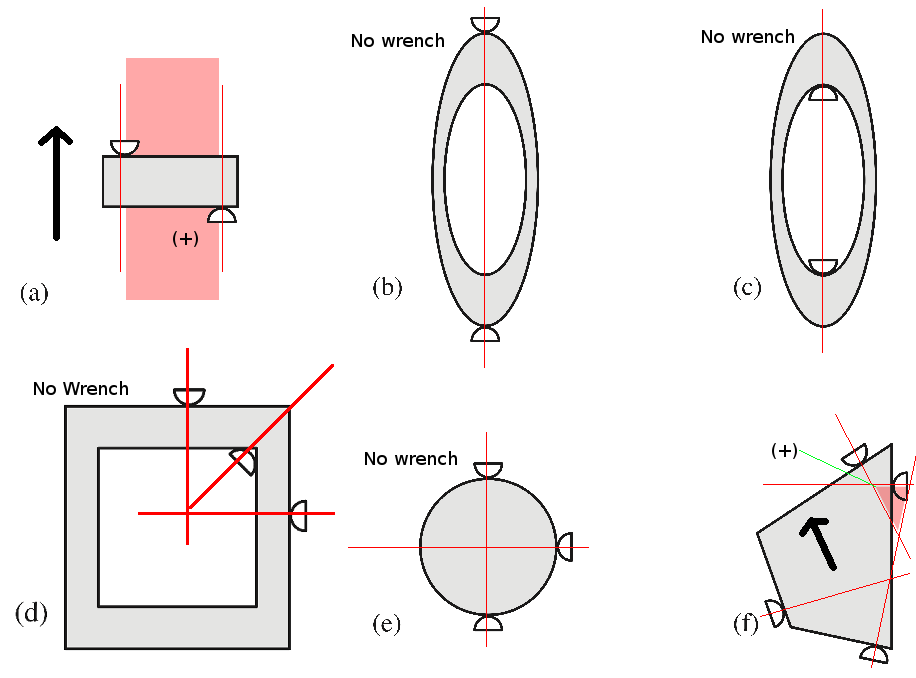
\includegraphics[width=\textwidth]{p1}
\caption{Contact scenarios showing the positive moment-labeled regions in red shading, with the contact normals rendered as bright red lines. An example acceptable wrench is rendered with a bold black arrow}
\label{fig:p1}
\end{figure}

\newpage

\section*{Problem 2}

\begin{figure}[h]
\centering
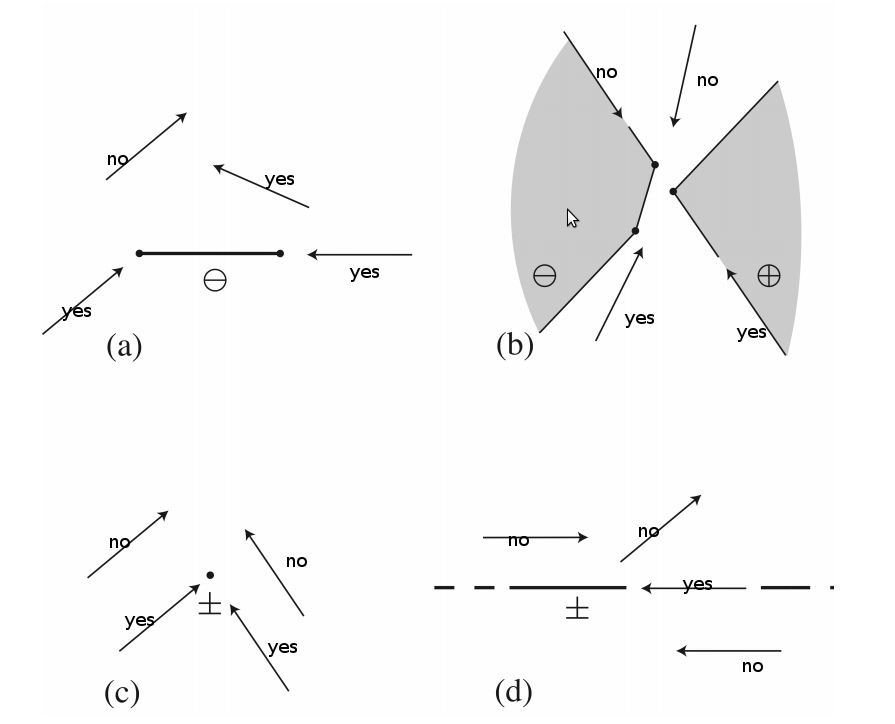
\includegraphics[width=\textwidth]{p2}
\caption{The acceptable wrenches are labeled along their arrows.}
\label{fig:p2}
\end{figure}

\newpage

\section*{Problem 3}

\begin{figure}[h]
\centering
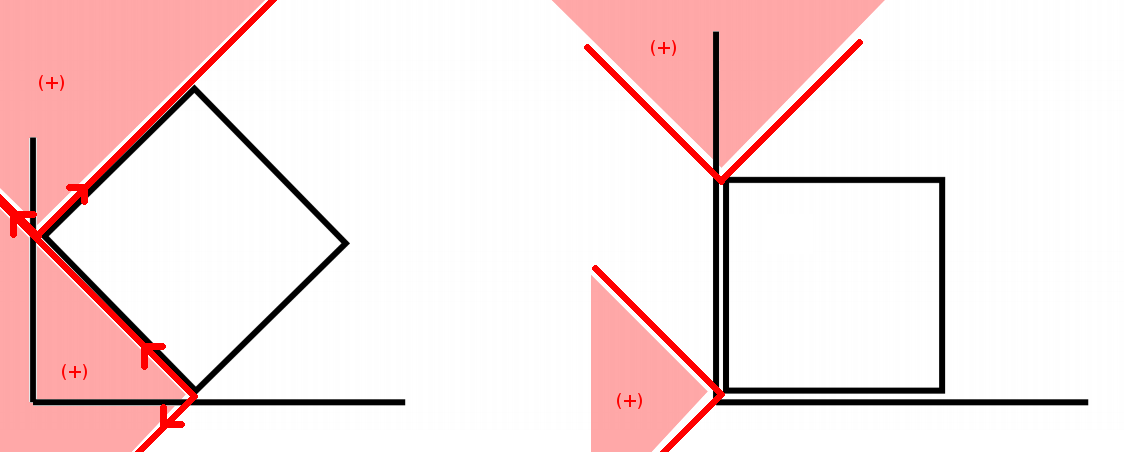
\includegraphics[width=\textwidth]{p3plus}
\caption{The positve moment labeled regions in the two subparts to the question. The collection of consistently labeled points lies along the line directed on the shared red edge.}
\label{fig:p3a}
\end{figure}

\begin{figure}[h]
\centering
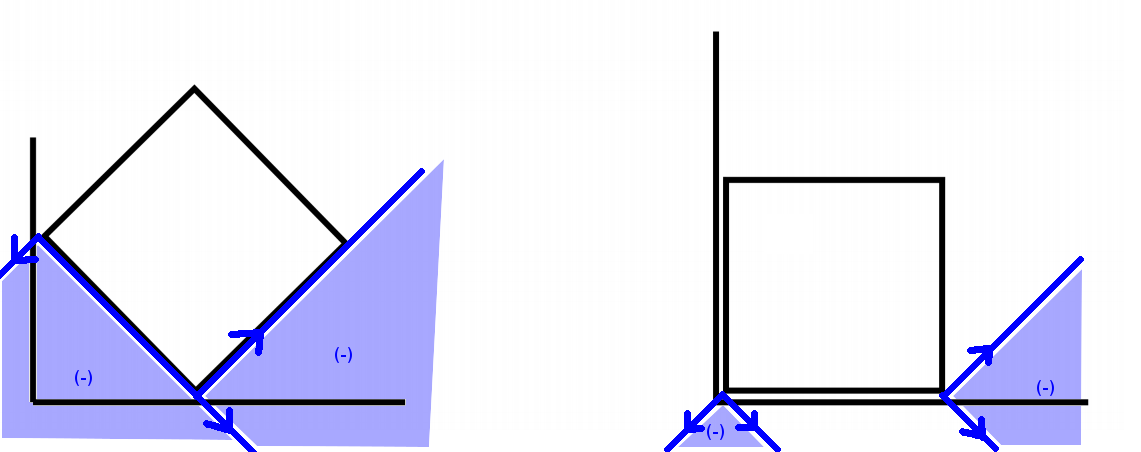
\includegraphics[width=\textwidth]{p3minus}
\caption{The negative moment labeled regions in the two subparts to the question. The collection of consistently labeled points lies along the line directed on the shared blue edge.}
\label{fig:p3b}
\end{figure}

\newpage

\section*{Problem 4}

\begin{figure}[h]
\centering
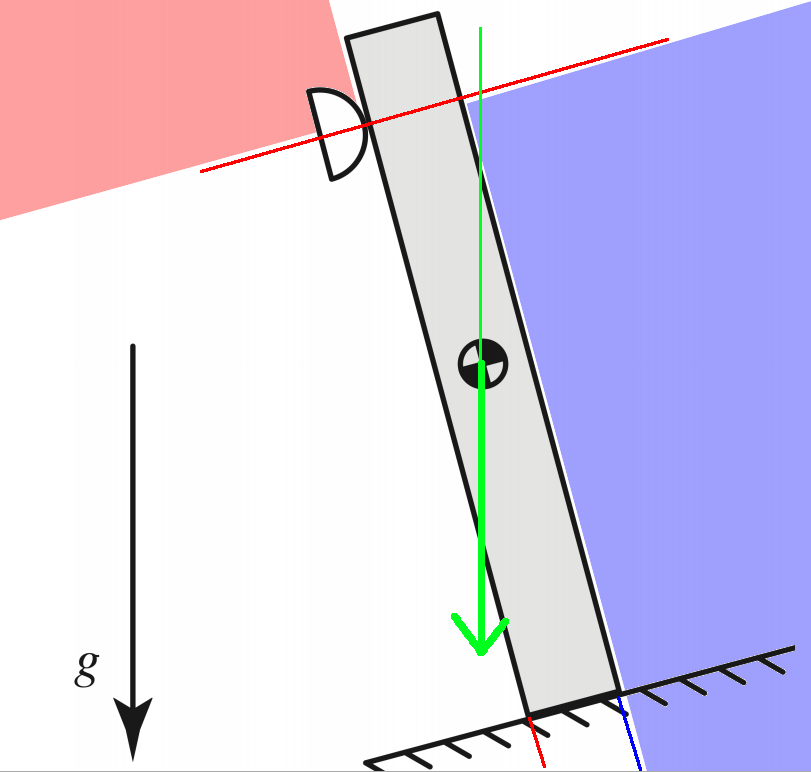
\includegraphics[width=\textwidth]{p4a}
\caption{The wrench applied by the gravity force on the object is rendered in green, showing that not all the points in the negative moment-labeling lie on its left hand side. Thus it is not in static balance.}
\label{fig:p4a}
\end{figure}

\begin{figure}[h]
\centering
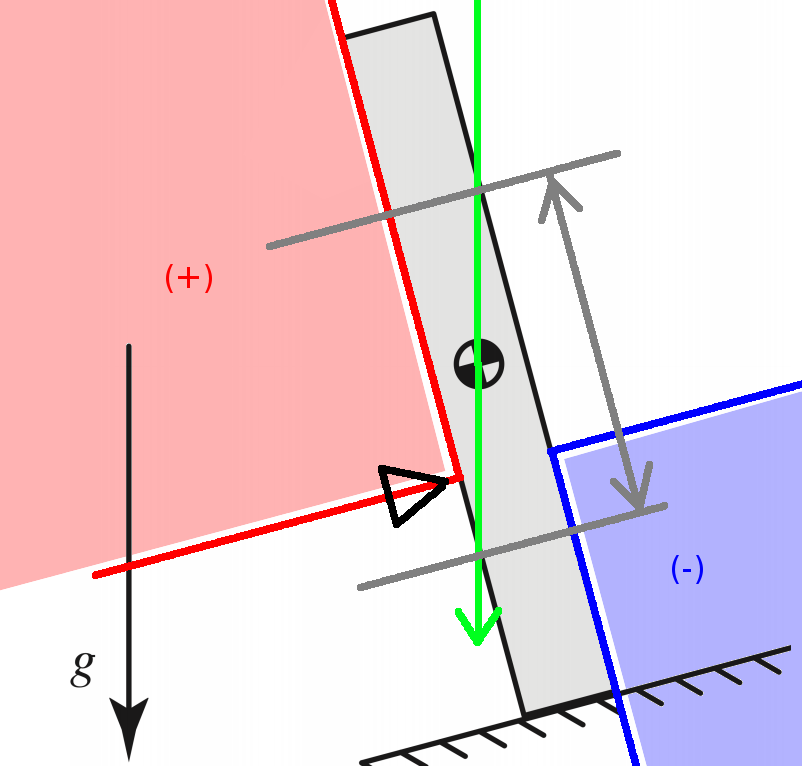
\includegraphics[width=\textwidth]{p4b}
\caption{By shifting the finger down, a range of contact positions keep the moment-labeled regions on seperate sides of the wrench applied by gravity, ensuring static balance. The gray marked region indicates the extents to which you may move the finger up and down along the left facing edge.}
\label{fig:p4b}
\end{figure}

\end{document}
